% Constructed and checked from the problem; not a geometric proof.
\documentclass[tikz,border=8pt]{standalone}
\begin{document}
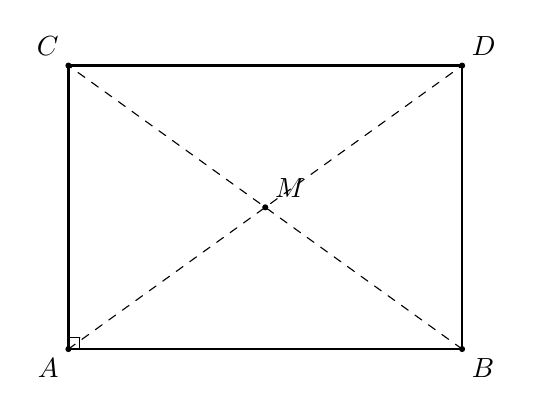
\begin{tikzpicture}[scale=1,line cap=round,line join=round]
\coordinate (p0) at (0,0);
\coordinate (p1) at (5,0);
\coordinate (p2) at (0,3.6);
\coordinate (p3) at (2.5,1.8);
\coordinate (p4) at (5,3.6);
\draw[thick] (p0) -- (p1);
\draw[thick] (p1) -- (p4);
\draw[thick] (p4) -- (p2);
\draw[thick] (p2) -- (p0);
\draw[dashed] (p0) -- (p4);
\draw[dashed] (p1) -- (p2);
\draw (0.1445,0) -- (0.1445,0.1445);
\draw (0.1445,0.1445) -- (0,0.1445);
\fill (p0) circle (1.1pt) node[below left] {$A$};
\fill (p1) circle (1.1pt) node[below right] {$B$};
\fill (p2) circle (1.1pt) node[above left] {$C$};
\fill (p3) circle (1.1pt) node[above right] {$M$};
\fill (p4) circle (1.1pt) node[above right] {$D$};
\end{tikzpicture}
\end{document}
